\section{The Type and Effect System}

\begin{frame}
\frametitle{The Type and Effect System}
\framesubtitle{Type Environments}
\begin{align}
    \Gamma; \Delta_1 \vdash e :: T \Delta_2
\end{align}
where
\begin{itemize}
    \item $\Gamma$ represents the type assumptions (is the type environment)
    \item $e$ is an expression of type $T$
    \item $\Delta_1, \Delta_2$ the lock status before and after the execution of expression $e$
\end{itemize}
\begin{align}
    \tag{Type Environment}
    \Gamma = \{x_1:T_1, x_2:T_2, ..., x_n:T_n\}
\end{align}
\end{frame}

\begin{frame}
\frametitle{The Type and Effect System}
\framesubtitle{Lock Environments}
\begin{align}
    \tag{Lock Environment}
    \Delta = \{a_1:n_1, a_2:n_2, ..., a_k:n_k\}
\end{align}
where
\begin{itemize}
    \item \textbf{$a_i$} represents a variable $x$ or a lock reference $r$
    \item \textbf{$n_i$} represents the lock's status which can be 0 for free locks or $n \ge 0$ which represents the number of times the lock is taken by the thread
\end{itemize}
\end{frame}


\begin{frame}
\frametitle{The Type and Effect System}
\framesubtitle{Notation}
\begin{align}
    \tag{Lock Environment Look-up}
    \Delta(a_i) = n_i
\end{align}
\begin{align}
    \tag{Type Environment Look-up}
    \Gamma(x_i) = T_i
\end{align}
\begin{align}
    \tag{Extending Lock Environment}
    \Delta, a_{k+1}:n_{k+1}
\end{align}
\begin{align}
    \tag{Extending Type Environment}
    \Gamma, x_{k+1}:T_{k+1}
\end{align}
\end{frame}


\begin{frame}
\frametitle{The Type and Effect System}
\framesubtitle{Notation}
\begin{align}
    \tag{Domain of Lock Environment}
    dom(\Delta) = \{a_1, a_2, ..., a_k\}
\end{align}
\begin{align}
    \tag{Domain of Type Environment}
    dom(\Gamma) = \{x_1, x_2, ..., x_n\}
\end{align}
\begin{align}
    \sigma; \Gamma; \Delta_1 \vdash e :: T \Delta_2 ~\text{where} ~\sigma~ \text{is the heap}
\end{align}
\end{frame}



\begin{frame}
\frametitle{The Type and Effect System}
\framesubtitle{Restriction}
The system disallows assignment to lock fields; imposes a single assignment policy for lock fields, which is assured in that we allow such assignments by the class constructors, only.
\end{frame}

\begin{frame}
\frametitle{The Type and Effect System}
\framesubtitle{Sum of Lock Environments}
\begin{definition}
Given two lock environments $\Delta_1, \Delta_2$, the sum of $\Delta_1 + \Delta_2 = \Delta$
\end{definition}
where
\begin{align}
    \Delta \vdash l:n_1+n_2 ~\text{if}~
    \Delta_1 \vdash l:n_1, 
    \Delta_2 \vdash l:n_2
\end{align}
\begin{align}
    \Delta \vdash l:n ~\text{if}~
    \Delta_1 \nvdash l, 
    \Delta_2 \vdash l:n
\end{align}
\begin{align}
    \Delta \vdash l:n ~\text{if}~
    \Delta_1 \vdash l:n, 
    \Delta_2 \nvdash l
\end{align}

\begin{align*}
    \Delta_1 \ge \Delta_2 ~\text{iff}~ dom(\Delta_1) \supseteq dom(\Delta_2) \wedge \forall l \in dom(\Delta_2), n_1 \ge n_2, \\
    ~\text{where}~ \Delta_1 \vdash l:n_1, 
    \Delta_2 \vdash l:n_2
\end{align*}
\end{frame}


\begin{frame}
\frametitle{The Type and Effect System}
\framesubtitle{Difference of Lock Environments}

\begin{prooftree}
\AxiomC{$\Delta_1 \vdash l:n_1$}
\AxiomC{$\Delta_2 \vdash l:n_2$}
\BinaryInfC{$\Delta_1-\Delta_2 \vdash l:n_1-n_2 $}
\end{prooftree}

\begin{prooftree}
\AxiomC{$\Delta + l$}
\AxiomC{$l \in dom(\Delta)$}
\AxiomC{$\Delta(l) = n$}
\TrinaryInfC{$\Delta \vdash l:n + 1 $}
\end{prooftree}

\begin{prooftree}
\AxiomC{$\Delta - l$}
\AxiomC{$l \in dom(\Delta)$}
\AxiomC{$\Delta(l) = n$}
\TrinaryInfC{$\Delta \vdash l:n - 1 $}
\end{prooftree}

\end{frame}


\begin{frame}
\frametitle{The Type and Effect System}
\framesubtitle{Aliases Problem}

The lock environments express resources (the current lock balance) and if $x$ and $y$ happen to be aliases, the resources must be combined.

\begin{align}
    x, y ~\text{not aliases}~ \rightarrow 
    \Delta' = \Delta [l1/x] [l2/y] = \{l1:1, l2:1\}
\end{align}
\begin{align}
    x, y ~\text{aliases}~ \rightarrow 
    \Delta' = \Delta [l/x] [l/y] = \{l:(1+1)\}
\end{align}
\end{frame}

\begin{frame}
\frametitle{The Type and Effect System}
\framesubtitle{Substitution}

\begin{definition}
Given a lock environment $\Delta$ the \textbf{substitution} of a variable x by a lock reference l in $\Delta$ is written as $\Delta[l/x]$. Let $\Delta' = \Delta [l/x]$
\end{definition}
\begin{prooftree}
\AxiomC{$\Delta' = \Delta'', l:n_l, x: n_x$}
\RightLabel{\textsc{COMP}}
\UnaryInfC{$\Delta' = \Delta'', l:(n_l + n_x)$}
\end{prooftree}

\begin{prooftree}
\AxiomC{$\Delta' = \Delta'', x:n$}
\AxiomC{$l \not \in dom(\Delta'')$}
\RightLabel{\textsc{REPL}}
\BinaryInfC{$\Delta' = \Delta'', l:n$}
\end{prooftree}
\end{frame}

\begin{frame}
    
\frametitle{The Type and Effect System}
\framesubtitle{Well-Formed Heaps}

$\sigma \vdash ok$ means the heap is well-formed, if no binding occurs more than once, and all references mentioned in the instance states are allocated in $\sigma$.

\end{frame}





\begin{frame}
\frametitle{The Type and Effect System}
\framesubtitle{Projection}

\begin{definition}
Assume a heap $\sigma$ with $\sigma \vdash ok$ and a thread $p$. The \textbf{projection} of $\sigma$ onto $p$, written $\sigma \downarrow_p$ is defined as:
\end{definition}
\begin{align*}
\bullet \downarrow_p & = \bullet \\
(\sigma, l:0) & = \sigma \downarrow_p l:0 \\
(\sigma, l:p(n))  & = \sigma \downarrow_p l:n \\
(\sigma, l:p'(n))  & = \sigma \downarrow_p l:0,  ~\text{if}~ p'\not = p \\
(\sigma, 0:C(\vec{v}))  & = \sigma \downarrow_p 
\end{align*}  
\end{frame}



\begin{frame}
\frametitle{The Type and Effect System}
\framesubtitle{Local Thread}
\begin{figure}[h]
    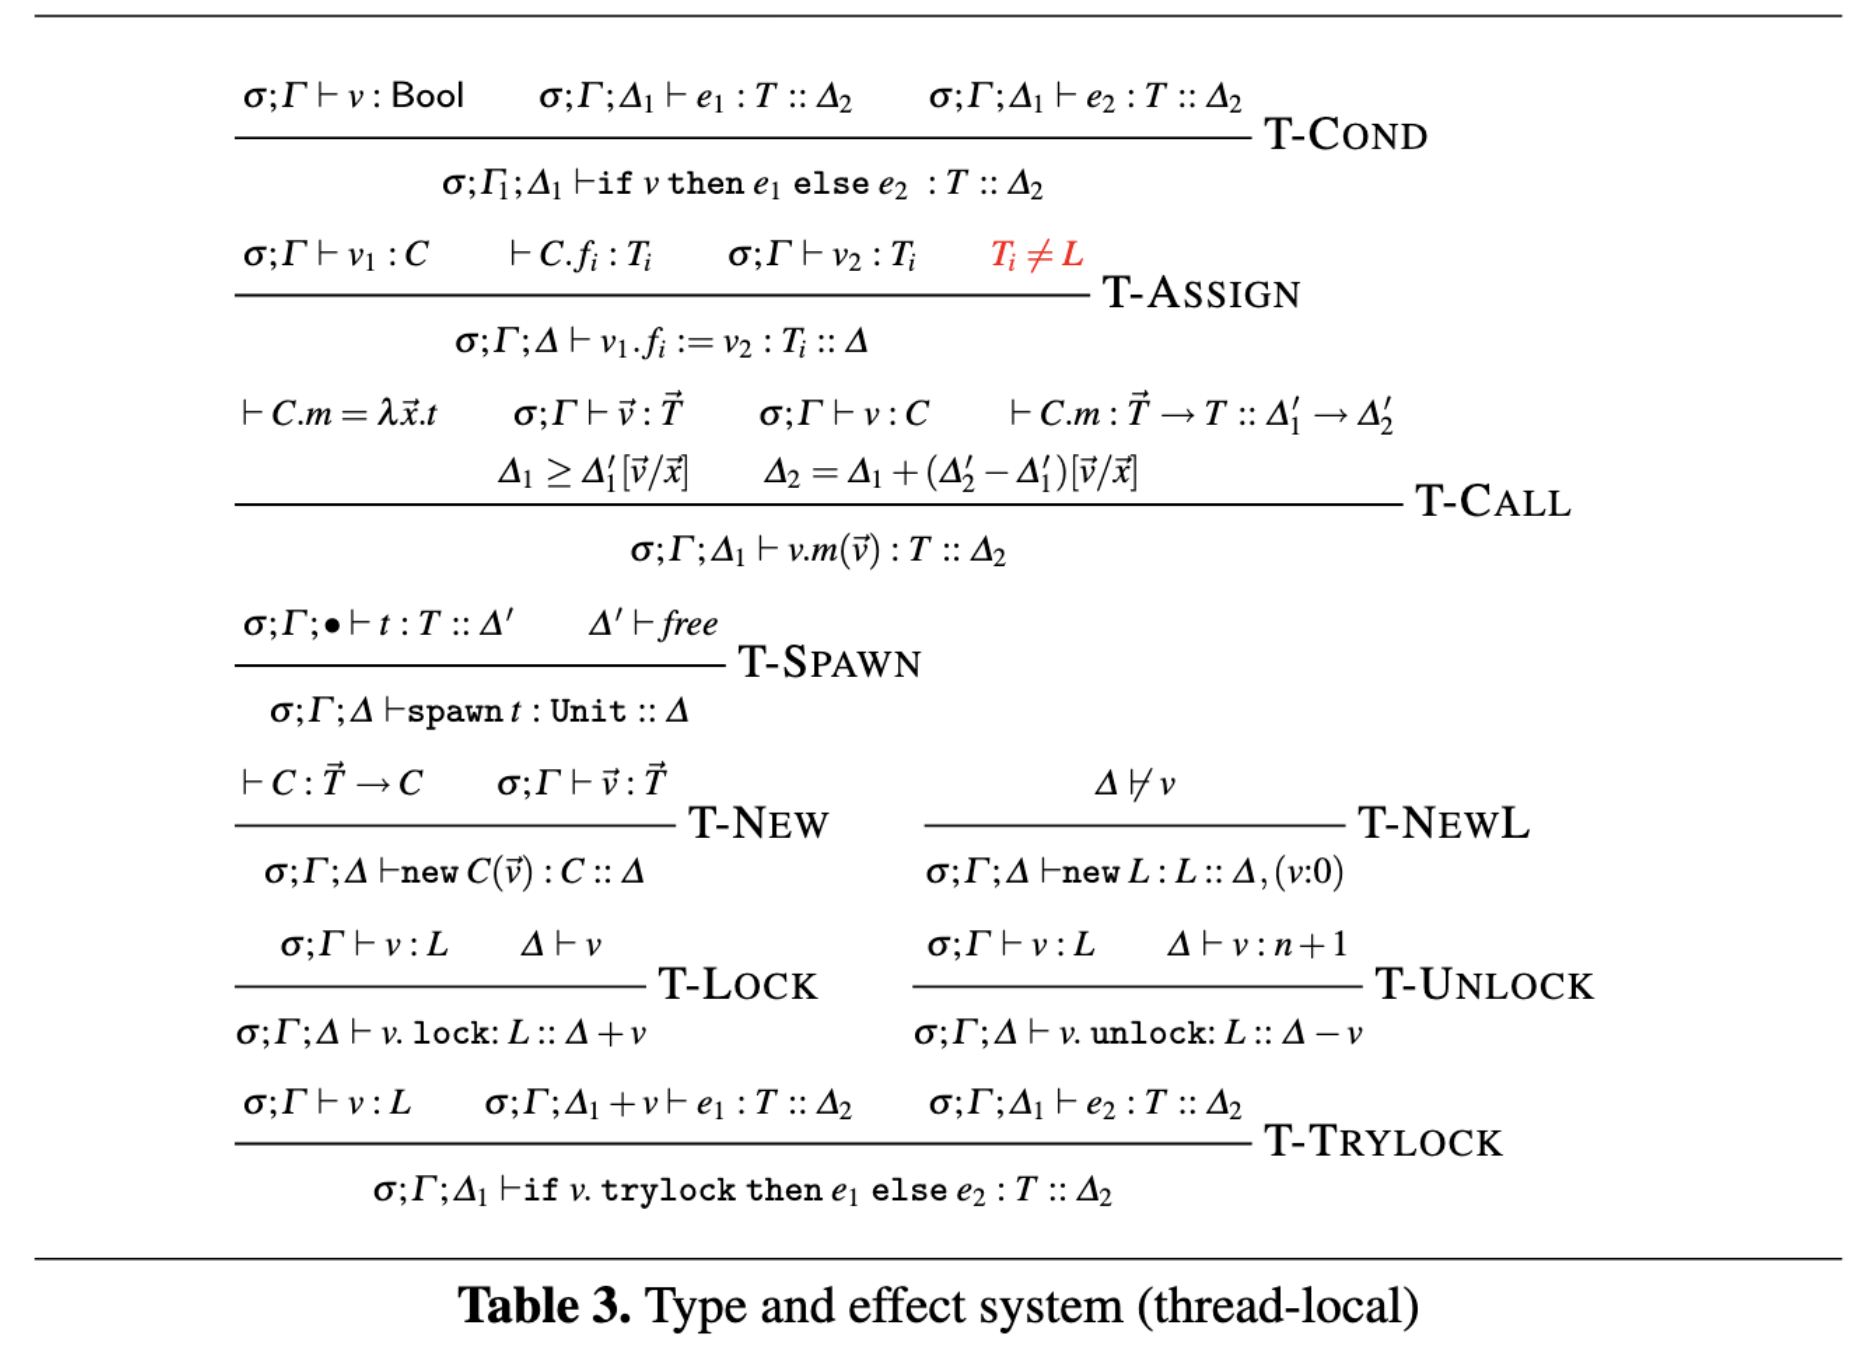
\includegraphics[width=10cm]{figures/local_system.png}
    \label{fig::local::system}
\end{figure}
\end{frame}



\begin{frame}
\frametitle{The Type and Effect System}
\framesubtitle{Global}
\begin{figure}[h]
    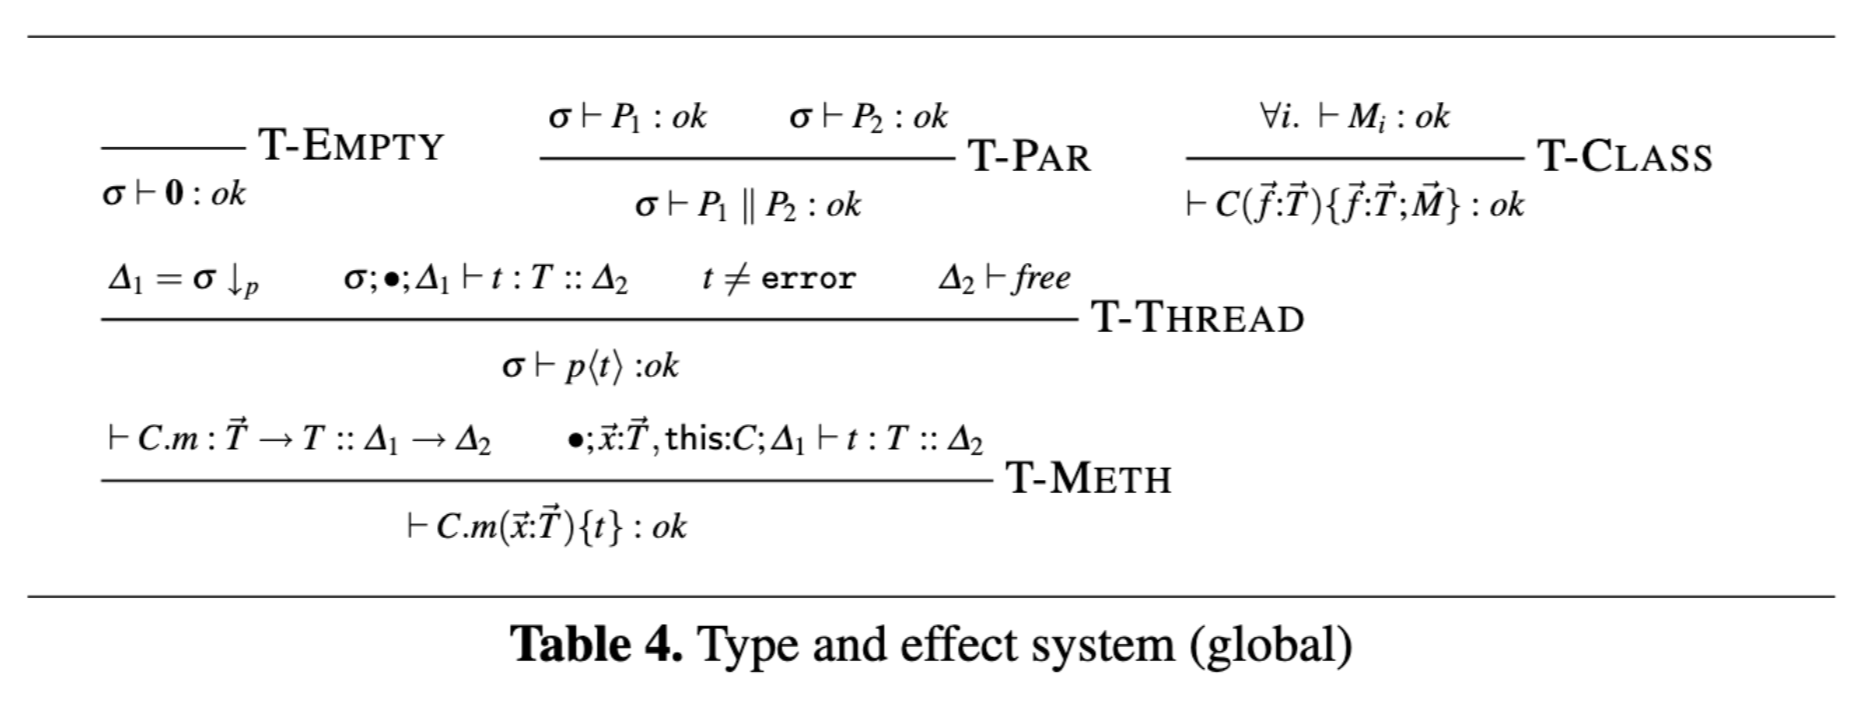
\includegraphics[width=10cm]{figures/global_system.png}
    \label{fig::global::system}
\end{figure}
\end{frame}

